\documentclass[addpoints]{exam}

% \usepackage{fancyhdr}
\usepackage[latin1]{inputenc}
\usepackage{amsmath}
\usepackage{amsfonts}
\usepackage{amssymb}
\usepackage{graphicx}
\usepackage[hmargin=2cm,vmargin=2.5cm]{geometry}
\usepackage[normalem]{ulem}
\usepackage{enumerate}



\begin{document}

\begin{center}
	\begin{large}
		MTH 201: Calculus, Spring/Summer 2015 \\
		Midterm Exam 1 --- Form A
		% Midterm Exam 1 --- Form B
	\end{large}
\end{center}

\noindent
\textbf{Instructions:} You may attempt as many of these problems as you wish. Any problem you do not attempt can be taken on a later Midterm Exam (as a different instance of the same problem). Your solutions \textbf{must be:}
\begin{itemize}
	\item Typewritten using correct mathematical notation and saved as a PDF, or 
	\item Neatly handwritten and scanned to a PDF (or handwritten on a tablet and saved as a PDF). 
\end{itemize}
Furthermore your solutions must conform to the specifications found in the \emph{Specifications for Student Work} document. Please review this document before submitting a final copy. \textbf{The PDF of your work must be uploaded to Blackboard at the appropriate place by 8:00pm EDT on Thursday, May 28.} No work will be accepted after this deadline unless you request a 24-hour extension using one of your tokens; requests for deadline extensions must be made by email (talbertr@gvsu.edu) and the new deadline will be 8:00pm EDT on Friday, May 29. 

\hrulefill

\begin{description}
	\item[Problem 0.] Consider the function, $f$, whose graph is given below: 
	\begin{center}
		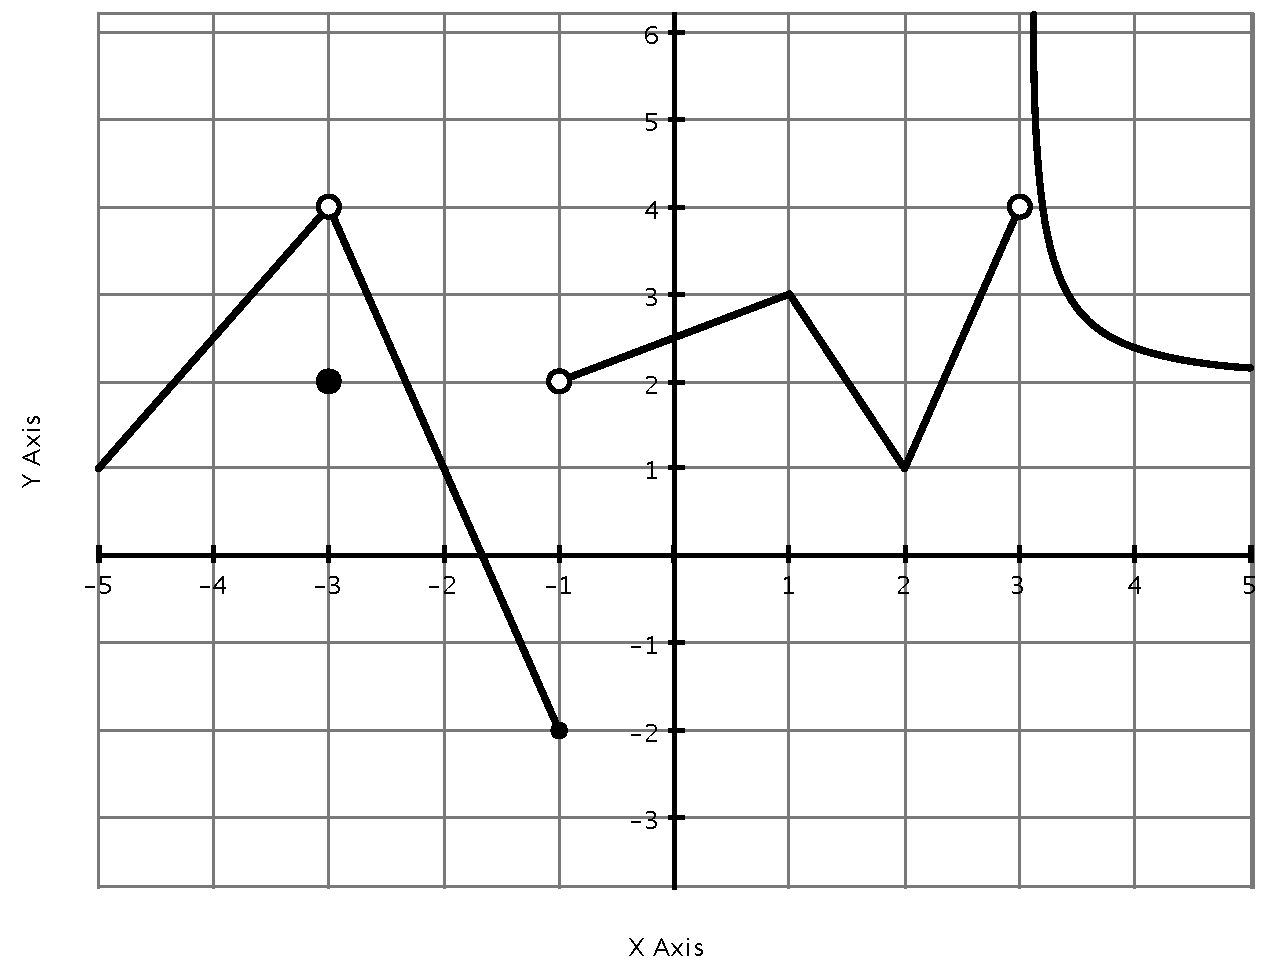
\includegraphics[width=0.5\textwidth]{examprob0a-1}
	\end{center}
	Using this graph, do the following:
	\begin{enumerate}
		\item State the value of $f(-3)$. If the function value fails to exist, say so and then explain why. 
		\item State the value of $\displaystyle{\lim_{x \to {-3}} f(x)}$. If the limit fails to exist, say so and then explain why. 
		\item State the value of $\displaystyle{\lim_{x \to {-1}} f(x)}$. If the limit fails to exist, say so and then explain why. 
		\item State the value of $\displaystyle{\lim_{x \to 1} f(x)}$. If the limit fails to exist, say so and then explain why. 	
		\item State the value of $\displaystyle{\lim_{x \to 3^-} f(x)}$. If the limit fails to exist, say so and then explain why. 	
		\item State the $x$-coordinates of the points where $f$ is discontinuous. 
		\item State the $x$-coordinates of the points where $f$ fails to be differentiable. 
	\end{enumerate}

% \begin{description}
% 	\item[Problem 0.] Consider the function, $f$, whose graph is given below: 
% 	\begin{center}
% 		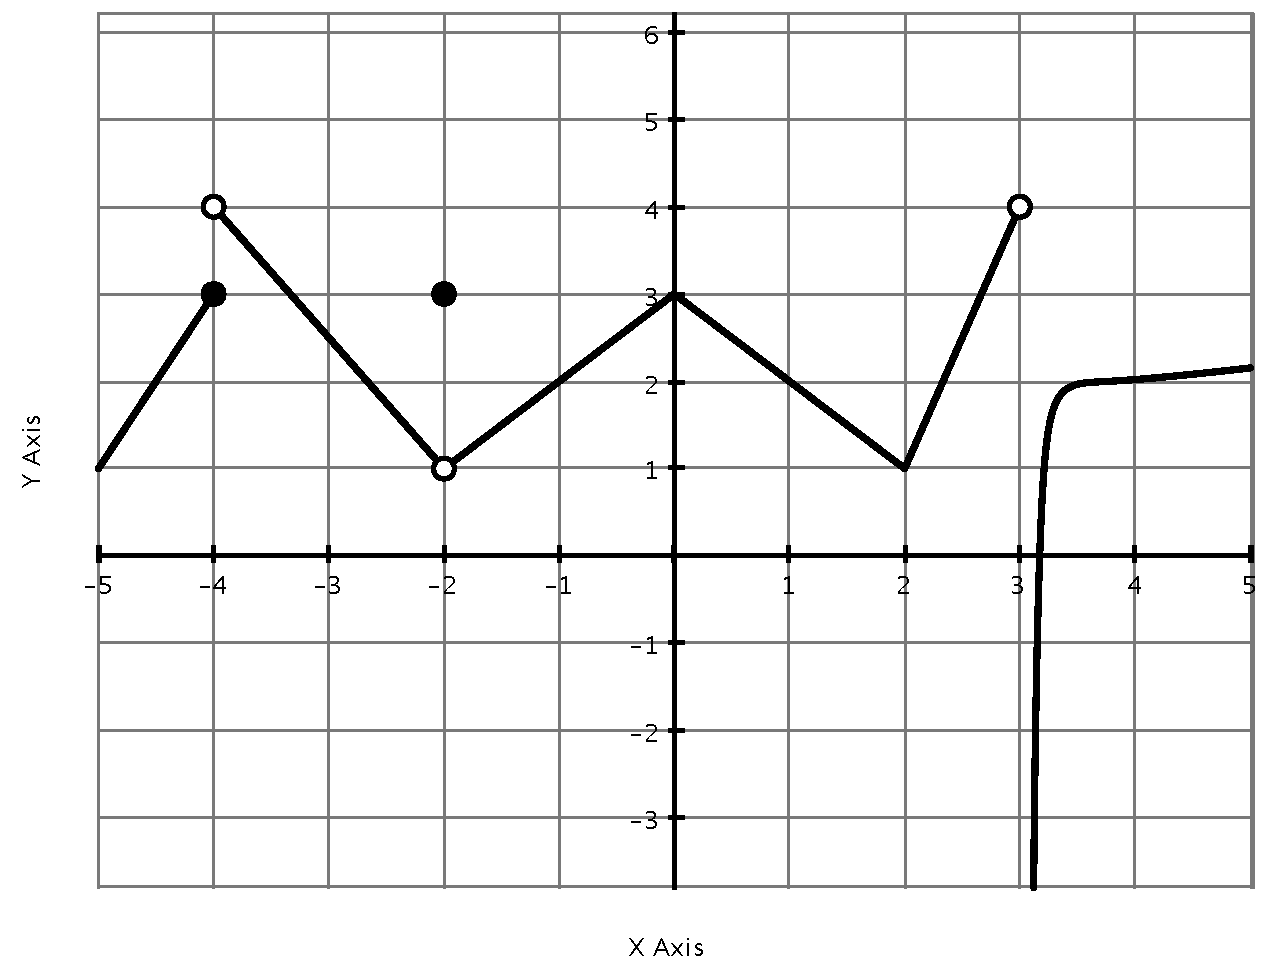
\includegraphics[width=0.5\textwidth]{examprob0b-1}
% 	\end{center}
% 	Using this graph, do the following:
% 	\begin{enumerate}
% 		\item State the value of $f(-4)$. If the function value fails to exist, say so and then explain why. 
% 		\item State the value of $\displaystyle{\lim_{x \to {-4}} f(x)}$. If the limit fails to exist, say so and then explain why. 
% 		\item State the value of $\displaystyle{\lim_{x \to {-2}} f(x)}$. If the limit fails to exist, say so and then explain why. 
% 		\item State the value of $\displaystyle{\lim_{x \to 0} f(x)}$. If the limit fails to exist, say so and then explain why. 	
% 		\item State the value of $\displaystyle{\lim_{x \to 3^-} f(x)}$. If the limit fails to exist, say so and then explain why. 	
% 		\item State the $x$-coordinates of the points where $f$ is discontinuous. 
% 		\item State the $x$-coordinates of the points where $f$ fails to be differentiable. 
% 	\end{enumerate}



\hrulefill

	\item[Problem 1.] The temperature $T$ (in degrees Fahrenheit) of a cake being baked in an oven $t$ minutes after being put into the oven is given by the formula 
	$$T(t) = 70 + 110(0.933)^t$$
	\begin{enumerate}
		\item Find the average rate of change in the cake's temperature over the first 15 minutes of being in the oven. Show all work and include correct units on your answer. 
		\item Write a limit expression that, if it were evaluated, would give the exact instantaneous rate of change in the cake's temperature exactly 15 minutes after being placed into the oven. 
		\item Evaluate the limit expression above to find the instantaneous rate of change in the cake's temperature exactly 15 minutes after being placed into the oven using a table of values. Show at least one sample calculation to illustrate how you constructed your table, and give a 1-2 sentence explanation of how you arrived at your answer. Also remember to put correct units on your answer. 
	\end{enumerate}



	% \item[Problem 1.] The number $T$ of tweets being sent out about a news event $t$ minutes after the event happens is modeled by the function 
	% $$T(t) = 100t^{2.5} (0.75)^t$$
	% \begin{enumerate}
	% 	\item Find the average rate of change in the number of tweets being sent during the first 5 minutes following the event. Show all work and include correct units on your answer. 
	% 	\item Write a limit expression that, if it were evaluated, would give the exact instantaneous rate of change in the number of tweets being exactly 5 minutes following the event. 
	% 	\item Evaluate the limit expression above to find the exact instantaneous rate of change in the number of tweets being exactly 5 minutes following the event using a table of values. Show at least one sample calculation to illustrate how you constructed your table, and give a 1-2 sentence explanation of how you arrived at your answer. Also remember to put correct units on your answer. 
	% \end{enumerate}


\hrulefill


	\item[Problem 2 \textbf{CORE}.] Consider the function $f(x) = x^3 - 3x^2 + x + 5$. 
		\begin{enumerate}
		\item Find the equation for the tangent line to the graph of this function at $x = 1$. Show all work, and use only the limit definition of the derivative. 
		\item Find the formula for the derivative of this function at any point. Show all work, and use only the limit definition of the derivative. 
		\end{enumerate}

	% \item[Problem 2 \textbf{CORE}.] Consider the function $f(x) = 2x^3 - x^2 + x + 2$. 
	% 	\begin{enumerate}
	% 	\item Find the equation for the tangent line to the graph of this function at $x = 1$. Use only the limit definition of the derivative. 
	% 	\item Find the formula for the derivative of this function at any point. Use only the limit definition of the derivative. 
	% 	\end{enumerate}


\hrulefill


	\item[Problem 3.] The table below shows the worldwide electric generating capacity of nuclear power plants, measured in gigawatts, over time: 
	\begin{center}
		\begin{tabular}{c||c|c|c|c|c|c|c|c|c}
		Year & 1960 & 1965 & 1970 & 1975 & 1980 & 1985 & 1990 & 1995 & 2000 \\ \hline
		Electric capacity & 1 & 5 & 16 & 71 & 135 & 250 & 328 & 340 & 347 
		\end{tabular}
	\end{center}
	\begin{enumerate}
		\item Use difference estimates to construct a table for the rate of change in electric capacity as a function of time. Show ALL work by hand, and do not use a spreadsheet. 
		\item Use a central difference estimate to approximate the second derivative of electric capacity in the year 1985. Show your work. 
		\item Looking at the values of the function, its first derivative, and its second derivative in 1985, give a 1-2 sentence that fully describes of the behavior of electric capacity in this year. Do not use the words \emph{function}, \emph{graph}, or \emph{derivative}, and make your explanation understandable to an average layperson. 
	\end{enumerate}

	% \item[Problem 3.] The density of human bones increases through childhood and adolescence. By age 18, 95\% of bone density has been achieved. The table below shows the percentage of maximum bone density achieved at different ages. 
	% \begin{center}
	% 	\begin{tabular}{c||c|c|c|c|c|c|c|c|c} 
	% 	Age (years) & 2 & 4 & 6 & 8 & 10 & 12 & 14 & 16 & 18 \\ \hline
	% 	Percentage of bone density & 43 & 49 & 51 & 56 & 63 & 71 & 82 & 91 & 95 
	% 	\end{tabular}
	% \end{center}
	% \begin{enumerate}
	% 	\item Use difference estimates to construct a table for the rate of change in percentage of bone density as a function of time. Show ALL work. 
	% 	\item Use a central difference estimate to approximate the second derivative of percentage of bone density at age 14. Show your work. 
	% 	\item Looking at the values of the function, its first derivative, and its second derivative at age 14, give a 1-2 sentence that fully describes of the behavior of percentage of bone density in this year. Do not use the words \emph{function}, \emph{graph}, or \emph{derivative}, and make your explanation understandable to an average layperson. 
	% \end{enumerate}

\end{description}

\end{document}